\documentclass[17pt]{extarticle}
\usepackage[landscape,scale=.9]{geometry}
\thispagestyle{empty}
\pagestyle{empty}
\usepackage{multicol}
\usepackage{amsmath}
\usepackage{fontspec}
\usepackage{unicode-math}
\setmainfont{TeX Gyre Pagella}
\setmathfont{TeX Gyre Pagella Math}

\usepackage{tikz}
\usetikzlibrary{calc,angles}
\usetikzlibrary{decorations.pathmorphing}
\usepackage{tikzducks}

\newcommand\qline{\tikz[dashed] \draw (0,0) -- +(3,0);}

\let\vec=\mathbf

%\url{https://tex.stackexchange.com/a/74613/86}
\usepackage{charter}
\usetikzlibrary{hobby,
  shapes.geometric,
  decorations,
  decorations.shapes,
  shapes.geometric,
  patterns
}

\makeatletter
\pgfdeclareradialshading[tikz@ball]{easter bg}{\pgfpoint{5bp}{25bp}}{%
color(0cm)=(tikz@ball!20);
color(0.15cm)=(tikz@ball!30);
color(0.4cm)=(tikz@ball!60);
color(0.9cm)=(tikz@ball)
}
\tikzoption{easter bg color}{\pgfutil@colorlet{tikz@ball}{#1}\def\tikz@shading{easter bg}\tikz@addmode{\tikz@mode@shadetrue}}


\pgfkeys{/tikz/easter star/.code args={#1 and #2}{
  \pgfdeclareradialshading[tikz@ball]{easter star}{\pgfpoint{#1}{#2}}{%
  color(0cm)=(tikz@ball!20);
  color(0.3cm)=(tikz@ball!40);
  color(0.65cm)=(tikz@ball!60);
  color(1cm)=(tikz@ball)
  }
 }
 \tikzoption{easter star color}{\pgfutil@colorlet{tikz@ball}{#1}\def\tikz@shading{easter star}\tikz@addmode{\tikz@mode@shadetrue}}
}

\makeatother

% original code by Paul Gaborit:
% tex.stackexchange.com/questions/72784/arrow-with-two-colors-with-tikz/#72793
\tikzset{
  double path/.style args={#1 colored by #2 and #3}{
    -,line join=round,line cap=rect,
    shorten >=0.1cm,
    shorten <=0.1cm,
    line width=#1,#2, % first path
    postaction={draw,-,#3,line width=(#1)/1.5,  
                shorten <=(#1)/3,shorten >=(#1)/3,
    }, % second path
  }
}

\tikzset{easter decoration 1/.style={
    decorate,
    decoration={
      shape backgrounds,
      shape=star,shape size=7pt,
      shape sep={0.5cm, between center},      
    },
    inner color=yellow,
    outer color=yellow!50!orange,
    draw=red!20!orange,
  }
}


\pgfdeclarepatternformonly{fivepointed stars easter 2}{\pgfpointorigin}{\pgfpoint{10mm}{10mm}}{\pgfqpoint{10mm}{8mm}}%
{
  \pgftransformshift{\pgfqpoint{1mm}{1mm}}
  \pgfpathmoveto{\pgfqpointpolar{18}{1mm}}
  \pgfpathlineto{\pgfqpointpolar{162}{1mm}}
  \pgfpathlineto{\pgfqpointpolar{306}{1mm}}
  \pgfpathlineto{\pgfqpointpolar{90}{1mm}}
  \pgfpathlineto{\pgfqpointpolar{234}{1mm}}
  \pgfpathclose%
  \pgfusepath{fill}
}

\tikzset{easter decoration 3/.style={
    draw=green!17!yellow,
    line width=2pt,
    star,
  }
}

\pgfdeclarepatternformonly{fivepointed stars easter 3}{\pgfpointorigin}{\pgfpoint{12mm}{12mm}}{\pgfqpoint{12mm}{11mm}}%
{
  \pgftransformshift{\pgfqpoint{1mm}{1mm}}
  \pgfpathmoveto{\pgfqpointpolar{18}{1mm}}
  \pgfpathlineto{\pgfqpointpolar{162}{1mm}}
  \pgfpathlineto{\pgfqpointpolar{306}{1mm}}
  \pgfpathlineto{\pgfqpointpolar{90}{1mm}}
  \pgfpathlineto{\pgfqpointpolar{234}{1mm}}
  \pgfpathclose%
  \pgfusepath{fill}
}

% * * * * * * * * * * * * * * * * * * * * * * * * * * * * * * * * * * * * * * * 

\begin{document}

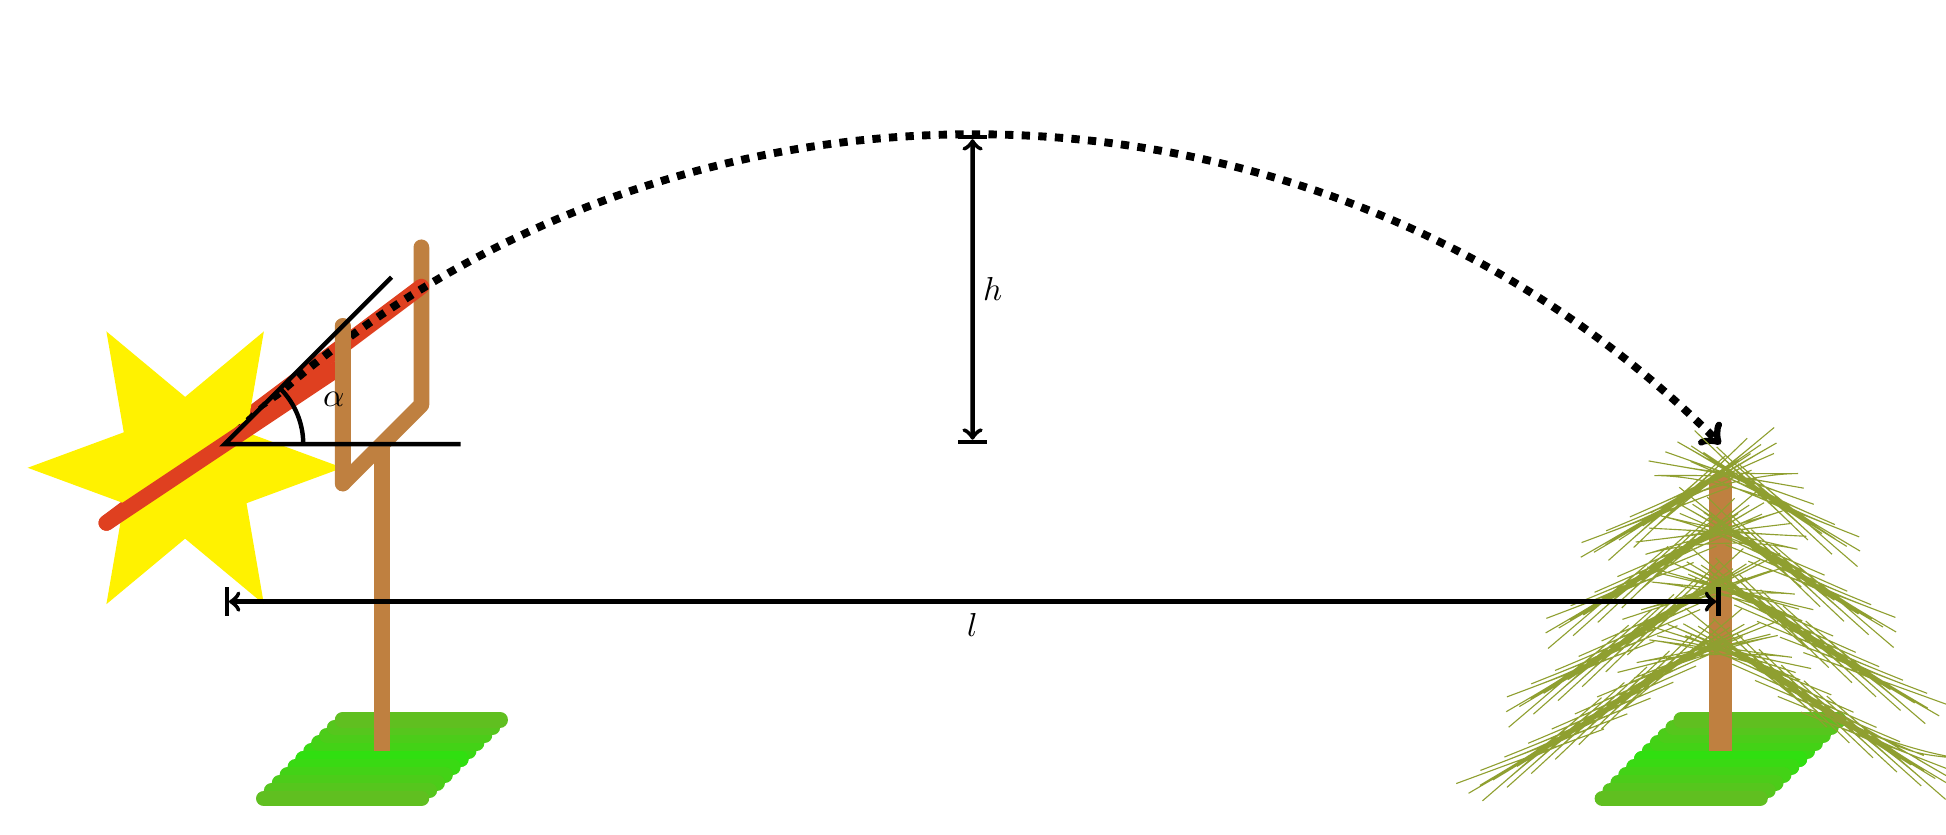
\begin{tikzpicture}[every node/.style={font=\large}]
\foreach[
  evaluate=\k as \tint using {5*(5-\k)+50},
  evaluate=\k as \xk using {\k/10}
  ] \k in {0,...,5} {
  \draw[line width=2mm, green!\tint!brown, line cap=round, line join=round] (0,-4) ++(\xk,\xk) ++(-1,0) -- +(2,0);
}
\draw[line width=2mm, brown, line cap=round, line join=round] (0,-4) -- (0,0) ++(-.5,-.5) +(0,2) -- coordinate[pos=.25](a) +(0,0) -- (.5,.5) --  coordinate[pos=.75](b) +(0,2);
\foreach[
  evaluate=\k as \tint using {5*(5-\k)+50},
  evaluate=\k as \xk using {\k/10}
  ] \k in {0,...,5} {
  \draw[line width=2mm, green!\tint!brown, line cap=round, line join=round] (0,-4) ++(-\xk,-\xk) ++(-1,0) -- +(2,0);
}
\path (a) ++(-3,-2) coordinate(c);
\draw[line width=2mm, red!50!brown, line cap=round, line join=round] (b) -- (c);
\path (c) ++(1,.7) coordinate (d);
\begin{scope}[shift=(d),rotate=30]
\fill[yellow] (90:2)  foreach \x in {1,...,12}
{
-- (90+\x*30:{2-1.1*mod(\x,2)})
};
\end{scope}


\draw[dashed,->,line width=1mm] (-2,0) to[out=45,in=135] coordinate(m) (17,0);
\draw[line width=2mm, red!50!brown, line cap=round, line join=round] (a) -- (c);
\draw[line width=2mm, brown, line cap=round, line join=round] (-.5,-.5) --  +(0,2);

\foreach[
  evaluate=\k as \tint using {5*(5-\k)+50},
  evaluate=\k as \xk using {\k/10}
  ] \k in {0,...,5} {
  \draw[line width=2mm, green!\tint!brown, line cap=round, line join=round] (17,-4) ++(\xk,\xk) ++(-1,0) -- +(2,0);
}
\draw[line width=3mm, brown, line cap=round] (17,-.5) -- ++(0,-3.5);
\foreach[
  evaluate=\k as \tint using {5*(5-\k)+50},
  evaluate=\k as \xk using {\k/10}
  ] \k in {0,...,5} {
  \draw[line width=2mm, green!\tint!brown, line cap=round, line join=round] (17,-4) ++(-\xk,-\xk) ++(-1,0) -- +(2,0);
}

\draw[rounded corners=10mm, green!25!brown,
           decorate,decoration={snake,amplitude=.1mm,segment length=10}]
    (16,-1) to[bend left,looseness=2] +(2,0)
    (15.5,-2) to[bend left,looseness=2] +(3,0)
    (15,-3) to[bend left,looseness=2] +(4,0)
    (14.5,-4) to[bend left,looseness=2] +(5,0)
    ;
    
    \draw[|<->|,ultra thick] (7.5,0) -- node[right] {\(h\)} (m);
    \draw[|<->|,ultra thick] (-2,-2) -- node[below] {\(l\)} (17,-2);
    \draw[ultra thick] (1,0) coordinate (A) -- (-2,0) coordinate(B) -- +(45:3) coordinate(C);
    \pic[draw, ultra thick, angle eccentricity=1.5,angle radius=1cm, pic text=\(\alpha\)] {angle};
\end{tikzpicture}

Initial speed \(u\) at angle \(\alpha\), acceleration \(-g\) vertically.

\begin{multicols}{2}

\begin{enumerate}
\item Initial velocity \(\vec{u} = \begin{pmatrix} \qline \\ \qline \end{pmatrix}\)
\item Vertical velocity \(v_y = \qline\)
\item Time to highest point \(t_m = \qline\)
\item Vertical position \(y = \qline\)
\item Height of highest point \(h = \qline\)
\item Time to landing \(t_l = \qline\)
\item Horizontal velocity \(v_x = \qline\)
\item Horizontal position \(x = \qline\)
\item Landing position \(l = \qline\)
\item Time in terms of horizontal position \(t = \qline\)
\item Vertical position in terms of horizontal position \(y = \qline\)
\end{enumerate}

\end{multicols}

\end{document}